\chapter{Vitesse de groupe, exclusion fermionique et mer de Dirac}

\section{Vitesse de phase et vitesse de groupe}

\begin{classroomqa}
\lecturetimestamp{00:00:07}
\audiencequestion{Qu’appelle-t-on vitesse de groupe et vitesse de phase ?}
\lecturerresponse{La vitesse de phase suit un point de phase constante dans une onde plane. En général, elle ne décrit pas le mouvement d’un objet mesurable. La vitesse de groupe suit l’enveloppe d’un paquet d’ondes ; c’est la vitesse associée aux particules, aux signaux et au flux de probabilité.}
\end{classroomqa}

Partons d’une onde plane,
\begin{equation}
\psi(x,t)=e^{i(kx-\omega t)},
\end{equation}
ou de sa forme réelle,
\begin{equation}
\psi(x,t)=\sin(kx-\omega t).
\end{equation}
Une crête, un creux ou tout autre point de phase constante se déplace de telle sorte que
\begin{equation}
kx-\omega t=\text{constant}.
\end{equation}
En choisissant, par commodité, la constante égale à zéro, on obtient
\begin{equation}
x=\frac{\omega}{k}t,
\qquad
v_{\mathrm{phase}}=\frac{\omega}{k}.
\end{equation}
Puisque \(\omega=2\pi/T\) et \(k=2\pi/\lambda\),
\begin{equation}
v_{\mathrm{phase}}=\frac{\omega}{k}=\frac{\lambda}{T}.
\end{equation}
Il s’agit simplement de la distance parcourue par une phase donnée pendant une période.

Pour une onde de Schr\"odinger non relativiste, avec \(\hbar=1\), l’énergie et la quantité de mouvement sont \(\omega\) et \(k\), d’où
\begin{equation}
\omega(k)=\frac{k^2}{2m}.
\end{equation}
Sa vitesse de phase est donc
\begin{equation}
v_{\mathrm{phase}}=\frac{k}{2m}.
\end{equation}
La vitesse ordinaire d’une particule de quantité de mouvement \(k\) est toutefois \(k/m\). Cet écart d’un facteur deux est le premier indice que le déplacement de la phase d’une onde plane n’est pas celui de la particule.

Un indice encore plus net apparaît. Ajoutons la même constante \(C\) à toutes les fréquences :
\begin{equation}
\omega(k)\longrightarrow \omega(k)+C.
\end{equation}
Cette constante pourrait, par exemple, représenter une contribution commune d’énergie au repos telle que \(mc_{\mathrm{light}}^2\), mais son nom précis importe peu. Ici, \(C\) est un décalage d’énergie, et non la vitesse de la lumière. La vitesse de phase devient
\begin{equation}
v_{\mathrm{phase}}\longrightarrow
\frac{\omega(k)+C}{k}
=v_{\mathrm{phase}}+\frac{C}{k}.
\end{equation}
Pourtant, ajouter la même constante à toutes les énergies ne change aucune différence d’énergie, et donc aucune propriété de la physique non relativiste.

On peut le voir directement dans la fonction d’onde. Écrivons un champ général de Schr\"odinger comme une somme ou une intégrale de modes,
\begin{equation}
\psi(x,t)=\sum_k a_k e^{ikx}e^{-i\omega(k)t},
\end{equation}
en laissant de côté les facteurs de normalisation. Après le décalage,
\begin{align}
\psi(x,t)
&\longrightarrow
\sum_k a_k e^{ikx}e^{-i[\omega(k)+C]t}
\\
&=e^{-iCt}\psi(x,t).
\end{align}
Chaque mode acquiert la même phase dépendant du temps. Le champ conjugué acquiert la phase opposée, de sorte que
\begin{equation}
\begin{aligned}
\psi^*(x,t)\psi(x,t)
&\longrightarrow
e^{iCt}e^{-iCt}\psi^*(x,t)\psi(x,t)
\\
&=\psi^*(x,t)\psi(x,t).
\end{aligned}
\end{equation}
La même annulation se produit dans les valeurs moyennes. Une grandeur qui change lorsque l’on décale le zéro de l’énergie ne peut pas être la vitesse physique de propagation de la particule de Schr\"odinger. La vitesse de phase dépend donc en partie d’une convention.

Une particule localisée est représentée non par une onde plane unique et infinie, mais par un paquet d’ondes. Les ondes qui le composent s’additionnent de façon constructive dans la région du paquet et destructive à l’extérieur. On peut déjà déterminer le mouvement de cette figure à partir de deux ondes voisines :
\begin{equation}
\psi(x,t)=
\sin(kx-\omega t)+
\sin(k'x-\omega't),
\end{equation}
où \(k'\) est proche de \(k\) et où \(\omega'=\omega(k')\). Les lieux d’interférence constructive sont ceux où leurs phases coïncident :
\begin{equation}
kx-\omega t=k'x-\omega't.
\end{equation}
Ainsi,
\begin{equation}
(k-k')x=(\omega-\omega')t,
\end{equation}
et le motif de renforcement se déplace selon
\begin{equation}
x=\frac{\omega-\omega'}{k-k'}t.
\end{equation}
En prenant la limite où les deux ondes deviennent voisines, on obtient
\begin{equation}
x=\frac{d\omega}{dk}t,
\qquad
v_{\mathrm{group}}=\frac{d\omega}{dk}.
\end{equation}
C’est la vitesse de l’enveloppe---, c’est-à-dire celle de la bosse localisée produite par l’interférence des ondes qui composent le paquet.

Pour la relation de dispersion non relativiste, avec le décalage arbitraire,
\begin{equation}
\omega(k)=\frac{k^2}{2m}+C,
\end{equation}
la vitesse de groupe vaut
\begin{equation}
v_{\mathrm{group}}
=\frac{d}{dk}\left(\frac{k^2}{2m}+C\right)
=\frac{2k}{2m}
=\frac{k}{m}.
\end{equation}
La constante additive a disparu, et le résultat est exactement la vitesse classique de la particule.

\begin{classroomqa}
\lecturetimestamp{00:16:35}
\audiencequestion{Le facteur deux disparaît-il dans la vitesse de groupe ?}
\lecturerresponse{Oui. La dérivation de \(k^2\) donne \(2k\), ce qui annule le facteur deux dans \(2m\). On obtient \(k/m\).}
\end{classroomqa}

La vitesse de groupe est donc celle qui est le plus étroitement associée au mouvement classique des particules. C’est aussi la vitesse pertinente pour la propagation d’un paquet et, dans les circonstances ordinaires considérées ici, pour celle des signaux. La vitesse de phase n’a pas nécessairement l’une ou l’autre de ces significations.

\subsection{Ondes relativistes massives et sans masse}

\begin{classroomqa}
\lecturetimestamp{00:17:47}
\audiencequestion{Cela a-t-il un rapport avec les affirmations selon lesquelles la lumière pourrait aller plus vite qu’elle-même ?}
\lecturerresponse{Non. Ces affirmations soulèvent une question distincte. Un calcul apparenté montre bien qu’une phase peut se déplacer plus vite que la lumière alors que la vitesse de groupe physique reste inférieure à celle-ci, mais cela ne décrit pas un signal qui devancerait la lumière.}
\end{classroomqa}

\begin{classroomqa}
\lecturetimestamp{00:18:05}
\audiencequestion{S’agit-il de l’exemple classique où la vitesse de phase dépasse celle de la lumière tandis que la vitesse de groupe reste inférieure ?}
\lecturerresponse{Oui. On retrouve le même comportement pour une onde relativiste de masse non nulle, et il découle directement de la relation relativiste énergie--quantité de mouvement.}
\end{classroomqa}

Posons \(\hbar=c_{\mathrm{light}}=1\). La relation relativiste est
\begin{equation}
E=\sqrt{p^2+m^2},
\qquad
\omega(k)=\sqrt{k^2+m^2}.
\end{equation}
Commençons par établir le cas sans masse. Lorsque \(m=0\),
\begin{equation}
\omega=|k|.
\end{equation}
Sur la branche se propageant vers la droite, \(k>0\), \(\omega=k\), et par conséquent
\begin{equation}
v_{\mathrm{phase}}=\frac{\omega}{k}=1,
\qquad
v_{\mathrm{group}}=\frac{d\omega}{dk}=1.
\end{equation}
Sur la branche se propageant vers la gauche, les deux vitesses ont le signe négatif correspondant. Dans les deux cas, leur valeur absolue est égale à la vitesse de la lumière. Comme la relation de dispersion est linéaire sur chacune des branches, toutes les composantes de Fourier de cette branche se déplacent à la même vitesse.

Pour une particule massive avec \(k>0\),
\begin{equation}
v_{\mathrm{phase}}
=\frac{\omega}{k}
=\sqrt{\frac{k^2+m^2}{k^2}}>1,
\end{equation}
tandis que
\begin{equation}
v_{\mathrm{group}}
=\frac{d\omega}{dk}
=\frac{k}{\sqrt{k^2+m^2}}<1.
\end{equation}
Pour \(k<0\), les deux vitesses changent de signe, mais leurs valeurs absolues satisfont aux mêmes inégalités. Ainsi, la phase peut se déplacer plus vite que la lumière tandis que le paquet, la particule, l’énergie et le signal se déplacent moins vite qu’elle. Pour cette relation de dispersion particulière et \(k\neq0\),
\begin{equation}
v_{\mathrm{phase}}v_{\mathrm{group}}=1.
\end{equation}
Cette relation inverse est une particularité de la relation de dispersion en racine carrée, et non une propriété générale des ondes.

\begin{figure}\centering
\includegraphics[width=0.72\textwidth]{lecture_05_figure_03.png}\caption{Relations de dispersion non relativiste et relativiste, avec la vitesse de phase \(\omega/k\) et la vitesse de groupe \(d\omega/dk\).}\lectureframe{00:35:52}\end{figure}

\begin{classroomqa}
\lecturetimestamp{00:23:41}
\audiencequestion{La dispersion est-elle liée au fait que la vitesse de l’onde dépend de sa fréquence ?}
\lecturerresponse{Oui. Lorsque \(\omega(k)\) est linéaire, toutes les composantes de Fourier ont la même vitesse de groupe, et le paquet peut conserver sa forme. Lorsque \(\omega(k)\) est non linéaire, les composantes se déplacent à des vitesses différentes ; le paquet se disperse et change de forme. Le son de basse fréquence est approximativement non dispersif lorsque sa fréquence est presque proportionnelle au nombre d’onde.}
\end{classroomqa}

En règle générale, la vitesse de phase ne transporte ni signal, ni énergie, ni flux de probabilité. Sa valeur numérique peut même être modifiée en décalant le zéro de l’énergie. La vitesse de groupe décrit le mouvement physiquement pertinent d’un paquet suffisamment étroit.

\begin{classroomqa}
\lecturetimestamp{00:25:14}
\audiencequestion{Peut-on mesurer la vitesse de phase d’un photon ?}
\lecturerresponse{Dans le vide, un photon a une relation de dispersion linéaire ; sa vitesse de phase et sa vitesse de groupe coïncident donc et sont toutes deux égales à la vitesse de la lumière. Dans un milieu matériel, la relation de dispersion change et les deux vitesses ne sont pas nécessairement égales.}
\end{classroomqa}

\begin{classroomqa}
\lecturetimestamp{00:25:50}
\audiencequestion{Cette discussion se limite-t-elle aux paquets d’ondes qui ne s’étalent pas au cours du temps ?}
\lecturerresponse{Un paquet ne conserve sa forme que si toutes ses composantes de Fourier ont la même vitesse, ce qui correspond à une relation de dispersion linéaire sur l’intervalle considéré. Avec une dispersion non linéaire, les composantes se séparent et le paquet s’étale.}
\end{classroomqa}

Les questions relatives aux cônes de lumière et à la structure causale relativiste exigent davantage que la distinction entre vitesse de phase et vitesse de groupe ; elles sont donc laissées de côté dans ce calcul.

\section{Symétrie par translation et lois de conservation}

Les phases des mêmes ondes planes permettent de présenter de façon concise les lois de conservation. Commençons par la conservation de l’énergie. Un champ d’annihilation agissant sur une particule incidente d’énergie \(\omega_j\) apporte un facteur temporel
\begin{equation}
e^{-i\omega_j t},
\end{equation}
tandis qu’un champ de création produisant une particule sortante d’énergie \(\omega'_r\) apporte
\begin{equation}
e^{+i\omega'_r t}.
\end{equation}
Pour plusieurs particules incidentes et sortantes, le produit de ces facteurs est
\begin{equation}
\exp\!\left[
i\left(\sum_r\omega'_r-\sum_j\omega_j\right)t
\right].
\end{equation}
Si l’interaction peut avoir lieu à n’importe quel instant avec la même amplitude, l’amplitude comporte une intégrale sur le temps d’interaction :
\begin{equation}
\begin{aligned}
&\int_{-\infty}^{\infty}dt\,
\exp\!\left[
i\left(\sum_r\omega'_r-\sum_j\omega_j\right)t
\right]
\\
&\quad =2\pi\,
\delta\!\left(\sum_r\omega'_r-\sum_j\omega_j\right).
\end{aligned}
\end{equation}
La fonction delta impose que l’énergie totale des particules sortantes soit égale à celle des particules incidentes. Une amplitude identique à chaque instant possible d’interaction exprime l’invariance par translation dans le temps et entraîne la conservation de l’énergie.

La translation dans l’espace entraîne la conservation de la quantité de mouvement par le même mécanisme. Considérons une désintégration physique en deux particules, où une particule incidente de quantité de mouvement \(k\) disparaît et où deux particules de quantités de mouvement \(k'_1\) et \(k'_2\) apparaissent. Une interaction locale au point \(x\) contient un champ d’annihilation et deux champs de création :
\begin{equation}
\mathcal{O}(x)=\psi^\dagger(x)\psi^\dagger(x)\psi(x).
\end{equation}
En omettant la dépendance temporelle et les facteurs de normalisation, les facteurs de mode pertinents sont
\begin{align}
\psi(x)&\supset a_k e^{ikx},
\\
\psi^\dagger(x)&\supset a_{k'_1}^\dagger e^{-ik'_1x},
\qquad
\psi^\dagger(x)\supset a_{k'_2}^\dagger e^{-ik'_2x}.
\end{align}
Dans l’élément de matrice
\begin{equation}
\langle k'_1,k'_2|\mathcal{O}(x)|k\rangle,
\end{equation}
l’opérateur d’annihilation élimine la particule incidente et les deux opérateurs de création fournissent les particules sortantes. Une fois ces actions des opérateurs effectuées, il reste le facteur dépendant de la position
\begin{equation}
e^{-ik'_1x}e^{-ik'_2x}e^{ikx}
=e^{i(k-k'_1-k'_2)x}.
\end{equation}
Comme aucun point n’est privilégié, on intègre sur toutes les positions possibles de désintégration :
\begin{equation}
\int_{-\infty}^{\infty}dx\,
e^{i(k-k'_1-k'_2)x}
=2\pi\delta(k-k'_1-k'_2).
\end{equation}
L’amplitude qui subsiste vérifie donc
\begin{equation}
k=k'_1+k'_2.
\end{equation}
En trois dimensions, le même calcul fait intervenir \(d^3x\), les vecteurs quantité de mouvement en gras et une fonction delta tridimensionnelle. Le raisonnement ne dépend pas du fait qu’il n’y ait qu’une particule incidente ou deux particules sortantes. Pour un nombre quelconque de particules, l’intégration sur le point d’interaction commun produit
\begin{equation}
\delta^{(3)}\!\left(
\sum_j\mathbf{k}_j-\sum_r\mathbf{k}'_r
\right).
\end{equation}
Une amplitude identique en tout point exprime l’invariance par translation dans l’espace et entraîne la conservation de la quantité de mouvement, tout comme une amplitude identique à chaque instant entraîne la conservation de l’énergie.

Un troisième exemple est une rotation globale de phase :
\begin{equation}
\psi\longrightarrow e^{i\lambda}\psi,
\qquad
\psi^\dagger\longrightarrow e^{-i\lambda}\psi^\dagger.
\end{equation}
L’amplitude d’interaction est invariante lorsque les phases apportées par les champs d’annihilation et de création s’annulent. Pour un champ porteur de charge électrique, cette égalité entre la charge retirée de l’état initial et celle rétablie dans l’état final exprime la conservation de la charge. Ainsi, les translations dans le temps, les translations dans l’espace et les rotations globales de phase montrent comment les champs qui créent et annihilent des particules encodent la conservation de l’énergie, de la quantité de mouvement et de la charge.

\begin{classroomqa}
\lecturetimestamp{00:37:52}
\audiencequestion{L’intégration sur l’espace signifie-t-elle qu’on intègre sur les trois dimensions spatiales ?}
\lecturerresponse{Oui. Les trois intégrales produisent une fonction delta pour les trois composantes de la quantité de mouvement ; les trois composantes de la quantité de mouvement totale sont donc conservées.}
\end{classroomqa}

\begin{classroomqa}
\lecturetimestamp{00:38:03}
\audiencequestion{Ce modèle détermine-t-il les probabilités relatives des différentes façons de répartir la quantité de mouvement conservée ?}
\lecturerresponse{Non. Cette expression simple impose la somme des quantités de mouvement sortantes, mais ne privilégie par ailleurs aucune répartition. Il faut des informations dynamiques supplémentaires pour déterminer les probabilités relatives.}
\end{classroomqa}

\begin{classroomqa}
\lecturetimestamp{00:39:04}
\audiencequestion{Pourquoi, dans une somme d’opérateurs d’annihilation, seul le terme correspondant au mode occupé subsiste-t-il ?}
\lecturerresponse{Un opérateur d’annihilation agissant sur un mode vide donne le vecteur nul. Si l’état ne contient qu’une particule, dans le mode \(k_0\), tous les termes s’annulent sauf celui pour lequel \(k=k_0\).}
\end{classroomqa}

Par exemple,
\begin{equation}
\sum_k a_k e^{ikx}|1_{k_0}\rangle
=e^{ik_0x}|0\rangle,
\end{equation}
à un facteur de normalisation près : tous les opérateurs d’annihilation associés à des modes vides donnent le vecteur nul.

\section{Amplification bosonique et exclusion fermionique}

Les bosons peuvent avoir tout nombre d’occupation entier positif ou nul dans un état à une particule, et leur algèbre de création favorise même un état déjà occupé. Pour un mode bosonique, la convention des états de nombre normalisés exprime l’amplification de l’occupation sous la forme\footnote{Le cours mentionne le facteur d’amplification en racine carrée de l’occupation ; cette équation indexée en donne la forme usuelle pour les états de nombre.}
\begin{equation}
a^\dagger|n\rangle=\sqrt{n+1}\,|n+1\rangle.
\end{equation}
Supposons qu’un atome excité puisse émettre un photon dans de nombreux modes possibles. En l’absence d’autres photons, les différentes directions et quantités de mouvement se présentent selon leur distribution de probabilité ordinaire. Si un mode particulier contient déjà de nombreux photons---tous de même quantité de mouvement, de même énergie et de même fréquence---, l’émission dans ce mode est amplifiée par le facteur correspondant, en racine carrée de l’occupation. L’atome a tendance à ajouter son photon à l’état déjà occupé. C’est l’émission stimulée, une manifestation concrète du regroupement des bosons.

Les fermions se comportent à l’inverse. Deux fermions identiques ne peuvent pas occuper le même état quantique. Le principe d’exclusion a d’abord été découvert en physique atomique, où deux électrons d’un atome ne peuvent pas avoir les mêmes nombres quantiques, mais il ne se limite pas aux atomes : des fermions identiques ne peuvent partager un état complet à une particule, où que ce soit.

Au départ, le développement du champ ressemble à celui des bosons. Dans une boîte de volume fini, on peut écrire
\begin{equation}
\psi(x)=\sum_k A_k e^{ikx},
\qquad
\psi^\dagger(x)=\sum_k A_k^\dagger e^{-ikx}.
\end{equation}
Pour une quantité de mouvement continue, les sommes deviennent des intégrales. Le signe opposé dans la phase spatiale conjuguée découle de la conjugaison hermitienne. Cette construction est non relativiste ; les fermions relativistes n’interviendront qu’à la fin.

L’état du champ est toujours décrit par un nombre d’occupation pour chaque mode, mais à présent chaque nombre ne peut valoir que zéro ou un :
\begin{equation}
|n_{k_1},n_{k_2},\ldots\rangle,
\qquad n_k\in\{0,1\}.
\end{equation}
Il n’existe pas d’autres types de particules relativistes qui autoriseraient, par exemple, au plus trois particules par état ou au moins sept particules par état. Établir que les statistiques bosoniques et fermioniques sont les seules possibilités exige la mécanique quantique et la relativité restreinte, et dépasse le cadre de cette discussion. Il s’agit ici de décrire le cas fermionique et ses conséquences.

\subsection{Un seul état fermionique}

Considérons un seul état à une particule. Il est soit vide, \(|0\rangle\), soit occupé, \(|1\rangle\). Les opérateurs de création et d’annihilation agissent comme suit :
\begin{align}
A^\dagger|0\rangle&=|1\rangle,
&
A^\dagger|1\rangle&=0,
\\
A|0\rangle&=0,
&
A|1\rangle&=|0\rangle.
\end{align}
Le zéro sans ornement à droite désigne le vecteur nul, et non l’état vide \(|0\rangle\). Tenter d’ajouter un second fermion ne donne pas le vide : cela ne produit aucun état physique.

\begin{classroomqa}
\lecturetimestamp{00:46:25}
\audiencequestion{Les opérateurs de création et d’annihilation fermioniques sont-ils toujours linéaires ?}
\lecturerresponse{Oui. Les opérateurs de mécanique quantique sont des opérateurs linéaires, y compris les opérateurs fermioniques de création et d’annihilation.}
\end{classroomqa}

\begin{classroomqa}
\lecturetimestamp{00:47:34}
\audiencequestion{Zéro désigne-t-il l’état vide ou signifie-t-il que l’opération tentée ne peut produire d’état ?}
\lecturerresponse{Il désigne le vecteur nul, et non l’état vide. Le véritable vide, ou état fondamental, a une fonction d’onde non nulle ; la fonction identiquement nulle a une norme nulle et n’est pas un état physique.}
\end{classroomqa}

L’oscillateur harmonique rend cette distinction concrète. Son état fondamental, c’est-à-dire l’état sans excitation de l’oscillateur, a une fonction d’onde gaussienne telle que
\begin{equation}
\phi_0(q)\propto e^{-\alpha q^2},
\qquad \alpha>0.
\end{equation}
C’est un état tout à fait acceptable et normalisable. En revanche,
\begin{equation}
\phi(q)\equiv0
\end{equation}
est le vecteur nul : il n’a aucune amplitude de probabilité, où que ce soit, et ce n’est pas un état. Ainsi, \(A^\dagger|1\rangle=0\) signifie que la seconde création tentée produit le vecteur nul.

\begin{classroomqa}
\lecturetimestamp{00:48:42}
\audiencequestion{Faut-il noter les opérateurs fermioniques différemment des opérateurs bosoniques ?}
\lecturerresponse{Oui. Il est plus clair de réserver \(a\) et \(a^\dagger\) aux modes bosoniques et d’utiliser \(c\) et \(c^\dagger\) pour les modes fermioniques. Les deux conventions se rencontrent dans la littérature, mais employer des lettres différentes permet de distinguer les deux algèbres.}
\end{classroomqa}

Avec cette notation, les règles pour un mode sont
\begin{align}
c^\dagger|0\rangle&=|1\rangle,
&c^\dagger|1\rangle&=0,
\\
c|0\rangle&=0,
&c|1\rangle&=|0\rangle.
\end{align}
Calculons maintenant les deux produits possibles sur chacun des états de base. Sur l’état vide,
\begin{align}
c^\dagger c|0\rangle&=0,
&
cc^\dagger|0\rangle&=|0\rangle.
\end{align}
Sur l’état occupé,
\begin{align}
c^\dagger c|1\rangle&=|1\rangle,
&
cc^\dagger|1\rangle&=0.
\end{align}
Leur somme redonne l’état sur lequel elle agit :
\begin{align}
(c^\dagger c+cc^\dagger)|0\rangle&=|0\rangle,
\\
(c^\dagger c+cc^\dagger)|1\rangle&=|1\rangle.
\end{align}
Comme \(|0\rangle\) et \(|1\rangle\) engendrent l’espace des états d’un mode,
\begin{equation}
c^\dagger c+cc^\dagger=1.
\end{equation}
La combinaison avec le signe plus est l’anticommutateur,
\begin{equation}
\{A,B\}=AB+BA,
\end{equation}
d’où la relation fermionique
\begin{equation}
\{c,c^\dagger\}=1.
\end{equation}
C’est l’analogue fermionique du commutateur bosonique
\begin{equation}
[a,a^\dagger]=aa^\dagger-a^\dagger a=1.
\end{equation}

Deux créations dans un même état fermionique donnent toujours zéro. Si l’état est vide, la première création le remplit et la seconde échoue ; s’il est déjà occupé, la première création échoue d’emblée. De même, deux annihilations donnent toujours zéro. Par conséquent,
\begin{equation}
\{c^\dagger,c^\dagger\}=2(c^\dagger)^2=0,
\qquad
\{c,c\}=2c^2=0.
\end{equation}

\begin{classroomqa}
\lecturetimestamp{00:56:45}
\audiencequestion{Le zéro dans la relation portant sur le carré de l’opérateur d’annihilation désigne-t-il un vecteur nul ?}
\lecturerresponse{L’équation affirme que \(c^2\) est l’opérateur nul. Cet opérateur envoie chaque vecteur d’état sur le vecteur nul. L’opérateur nul et le vecteur nul sont des objets mathématiques distincts, bien que le premier produise toujours le second.}
\end{classroomqa}

Pour plusieurs modes discrets de quantité de mouvement, l’algèbre complète est
\begin{align}
\{c_k,c_{k'}^\dagger\}&=\delta_{kk'},
\\
\{c_k,c_{k'}\}&=0,
\\
\{c_k^\dagger,c_{k'}^\dagger\}&=0.
\end{align}
Le delta de Kronecker vaut un lorsque \(k=k'\) et zéro sinon. Pour les quantités de mouvement continues, on le remplace, avec la normalisation appropriée, par une fonction delta de Dirac. Les anticommutateurs entre opérateurs de même type s’annulent pour toute paire de modes, et pas seulement lorsque leurs indices coïncident.

\subsection{Exclusion dans l’espace des positions}

L’algèbre indexée par la quantité de mouvement affirme d’abord que deux fermions identiques d’une même espèce ne peuvent occuper un même mode de quantité de mouvement. Elle va plus loin. Une particule localisée en position \(x\) est créée par
\begin{equation}
\psi^\dagger(x)=\sum_k c_k^\dagger e^{-ikx},
\end{equation}
à un facteur de normalisation près. À l’origine, tenter de créer deux particules donne
\begin{align}
\psi^\dagger(0)\psi^\dagger(0)|\Omega\rangle
&=\sum_{k,k'}c_k^\dagger c_{k'}^\dagger|\Omega\rangle.
\end{align}
Les indices \(k\) et \(k'\) sont des variables muettes de sommation. Permuter ces indices laisse la somme double inchangée ; on peut donc en prendre la moyenne avec son expression où les indices sont permutés :
\begin{align}
\sum_{k,k'}c_k^\dagger c_{k'}^\dagger|\Omega\rangle
&=\frac12\sum_{k,k'}
\left(c_k^\dagger c_{k'}^\dagger
+c_{k'}^\dagger c_k^\dagger\right)|\Omega\rangle
\\
&=\frac12\sum_{k,k'}
\{c_k^\dagger,c_{k'}^\dagger\}|\Omega\rangle
=0.
\end{align}

\begin{classroomqa}
\lecturetimestamp{01:02:26}
\audiencequestion{Dans la somme de deux particules en position, seuls les termes de quantités de mouvement différentes s’annulent-ils ?}
\lecturerresponse{Non. La permutation des indices muets transforme toute la somme double en la moitié de l’anticommutateur de deux opérateurs de création. Cet anticommutateur s’annule pour toute paire de quantités de mouvement ; la somme entière est donc nulle.}
\end{classroomqa}

Le calcul montre que l’exclusion ne concerne pas seulement les états propres de quantité de mouvement. Des fermions identiques ne peuvent pas non plus être placés dans un même état de position. Plus généralement, ils ne peuvent occuper aucun état identique à une particule.

\subsection{Qu’est-ce qui définit un même état ?}

\begin{classroomqa}
\lecturetimestamp{01:04:30}
\audiencequestion{Deux électrons très éloignés l’un de l’autre peuvent-ils avoir la même quantité de mouvement ?}
\lecturerresponse{L’exclusion porte sur l’état complet à une particule. Deux électrons peuvent avoir la même valeur propre exacte de quantité de mouvement si un autre indice compatible, comme le spin, diffère. Les électrons spatialement séparés sont plutôt des paquets localisés que des états propres exacts de quantité de mouvement ; leurs quantités de mouvement moyennes peuvent être presque égales alors que leurs fonctions d’onde spatiales restent distinctes. Ce qui est interdit, c’est l’identité des états complets.}
\end{classroomqa}

Le spin n’a pas encore été étudié, mais il fournit un indice supplémentaire familier. Deux électrons peuvent avoir la même valeur de quantité de mouvement si leurs états de spin diffèrent. Une fois pris en compte tous les indices pertinents, deux fermions identiques ne peuvent partager le même état complet.

\begin{classroomqa}
\lecturetimestamp{01:05:25}
\audiencequestion{Les électrons de deux atomes d’hydrogène séparés peuvent-ils avoir la même quantité de mouvement ou le même état atomique ?}
\lecturerresponse{Un électron lié dans un atome n’est pas un état propre de quantité de mouvement. Sa fonction d’onde orbitale est centrée sur cet atome. Deux atomes séparés peuvent chacun avoir un électron dans ce qu’on appelle l’état fondamental atomique, mais une orbitale est centrée sur le premier atome et l’autre sur le second ; ce sont donc deux états à une particule différents.}
\end{classroomqa}

\begin{classroomqa}
\lecturetimestamp{01:06:33}
\audiencequestion{Peut-on remplacer le terme plus général « système » par « état » ?}
\lecturerresponse{Non. Un système est un ensemble de degrés de liberté ; un état spécifie une configuration quantique particulière de ce système. Un électron est un système, tandis que sa fonction d’onde orbitale et de spin décrit un état de ce système.}
\end{classroomqa}

\begin{figure}\centering
\includegraphics[width=0.74\textwidth]{lecture_05_figure_04.png}\caption{Fonctions d’onde localisées à une particule et état créé par deux opérateurs de création, utilisé pour examiner l’exclusion fermionique.}\lectureframe{01:07:21}\end{figure}

\begin{classroomqa}
\lecturetimestamp{01:07:22}
\audiencequestion{Un faisceau d’électrons dans un tube cathodique ne contient-il jamais deux électrons dans le même état ?}
\lecturerresponse{Oui. Les électrons occupent des paquets d’ondes distincts, séparés dans l’espace ou distingués d’une autre façon dans leurs états complets. C’est le contraire des photons, qui peuvent tous occuper le même mode d’onde plane et former un faisceau cohérent.}
\end{classroomqa}

On peut se représenter un faisceau d’électrons comme un paquet localisé suivi d’un autre. Les paquets n’ont pas besoin d’être des états exacts de position ou de quantité de mouvement ; il suffit que leurs fonctions d’onde soient distinctes. Un faisceau de photons, en revanche, peut contenir de nombreux photons dans un seul et même état d’onde plane.

\begin{classroomqa}
\lecturetimestamp{01:08:14}
\audiencequestion{Deux électrons peuvent-ils se trouver à la même position avec des quantités de mouvement différentes ?}
\lecturerresponse{La position exacte et la quantité de mouvement exacte sont des indices incompatibles, car les opérateurs correspondants ne commutent pas. On ne peut pas spécifier un état à une particule par une position et une quantité de mouvement simultanément bien définies. Dans ce cadre non relativiste, le spin peut accompagner un indice de position ou de quantité de mouvement, car il commute avec ces observables.}
\end{classroomqa}

\begin{classroomqa}
\lecturetimestamp{01:08:51}
\audiencequestion{Les électrons liés et séparés sont-ils approximativement dans des états de position ?}
\lecturerresponse{Ce ne sont pas des états propres exacts de position, puisque chaque orbitale a une étendue spatiale finie, mais chacun est approximativement localisé près de son propre atome. Cette localisation suffit à rendre leurs fonctions d’onde orbitales distinctes.}
\end{classroomqa}

\begin{classroomqa}
\lecturetimestamp{01:09:31}
\audiencequestion{Quelle est la définition d’un état quantique ?}
\lecturerresponse{Un état est l’analogue quantique de la configuration d’un système. Il contient les informations nécessaires pour attribuer des probabilités aux différentes mesures possibles. Pour un électron, l’état est représenté par une fonction d’onde, à laquelle s’ajoutent les éventuels indices internes tels que le spin.}
\end{classroomqa}

\begin{classroomqa}
\lecturetimestamp{01:10:32}
\audiencequestion{Des électrons localisés en des lieux très éloignés peuvent-ils être dans le même état ou avoir la même quantité de mouvement ?}
\lecturerresponse{Ils ne peuvent pas être dans le même état, car leur localisation diffère : un électron ici et un autre dans la galaxie d’Andromède, ou l’un au Nevada et l’autre dans le Connecticut, ont des fonctions d’onde distinctes. Leurs quantités de mouvement peuvent être presque égales. Rendre la quantité de mouvement de l’un ou l’autre infiniment précise étalerait sa fonction d’onde dans tout l’espace et supprimerait la localisation qui distinguait les états.}
\end{classroomqa}

La forme de la relation d’incertitude position--quantité de mouvement exprimée en écarts-types est
\footnote{Le cours énonce qualitativement le produit d’incertitude ; le facteur \(\hbar/2\) est donné par la convention en écarts-types.}
\begin{equation}
\Delta x\,\Delta p\geq\frac{\hbar}{2}.
\end{equation}
Un paquet peut être localisé au Nevada et avoir une distribution de quantité de mouvement assez étroite, tandis qu’un autre paquet, dans le Connecticut, a une distribution presque identique. Ils restent des états distincts parce que leurs fonctions d’onde spatiales diffèrent. À la limite d’un état propre exact de quantité de mouvement, aucun des deux paquets ne reste localisé en l’un ou l’autre lieu.

Les opérateurs fermioniques s’utilisent dans les réactions de la même façon que les opérateurs bosoniques. Un opérateur d’annihilation d’électron élimine un électron incident, un opérateur de création d’électron fournit un électron sortant, et ces facteurs peuvent être multipliés par des opérateurs de création ou d’annihilation de photons. Les photons sont des bosons, tandis que les électrons sont des fermions. Les produits de leurs opérateurs servent à comptabiliser les réactions comprenant des électrons incidents et sortants, ainsi que des photons émis ou absorbés.

\begin{classroomqa}
\lecturetimestamp{01:13:36}
\audiencequestion{L’exclusion de Pauli est-elle communiquée localement, ou s’impose-t-elle globalement lorsque deux processus de création sont spatialement séparés ?}
\lecturerresponse{Si l’on sait qu’une particule se trouve au Nevada et l’autre dans le Connecticut, elles ne sont pas dans le même état.}
\end{classroomqa}

\editorialnote{Une courte partie de la réponse à cette question n’a pas pu être récupérée. La distinction entre les états localisés à une particule et les superpositions Nevada--Connecticut est établie.}

Lorsque leur position n’est pas déterminée, la question de l’exclusion est de savoir si les fonctions d’onde complètes à une particule coïncident. Les superpositions Nevada--Connecticut rendent cette distinction explicite.

Soient \(|N\rangle\) et \(|C\rangle\) deux états orthonormés localisés respectivement au Nevada et au Connecticut. On a
\begin{equation}
|+\rangle=\frac{|N\rangle+|C\rangle}{\sqrt2},
\qquad
|-\rangle=\frac{|N\rangle-|C\rangle}{\sqrt2}.
\end{equation}
L’état \(|+\rangle\) attribue des probabilités égales à la présence de son unique électron au Nevada et au Connecticut. L’état \(|-\rangle\) donne les mêmes probabilités de position, mais s’en distingue par une phase relative. Les deux états sont orthogonaux :
\begin{equation}
\langle+|-\rangle=0.
\end{equation}
Deux électrons ne peuvent pas occuper tous deux \(|+\rangle\), ni tous deux \(|-\rangle\), mais le principe d’exclusion n’empêche pas que l’un occupe chaque état.

\begin{classroomqa}
\lecturetimestamp{01:16:25}
\audiencequestion{Un électron peut-il occuper la superposition, avec un signe plus, du Nevada--et du Connecticut, et un autre la superposition avec un signe moins ?}
\lecturerresponse{Oui. Les combinaisons avec les signes plus et moins sont orthogonales et constituent donc des états à une particule distincts.}
\end{classroomqa}

\begin{classroomqa}
\lecturetimestamp{01:16:39}
\audiencequestion{L’exemple des états séparés suppose-t-il une notion de simultanéité ?}
\lecturerresponse{Le modèle considéré ici est non relativiste. Il compare les deux états occupés sur une même tranche de temps, avec un temps absolu commun aux régions du Nevada et du Connecticut, pourtant séparées dans l’espace. Il néglige aussi les limites opérationnelles dues à la vitesse finie à laquelle on peut comparer ces régions. La physique relativiste introduit un certain flou dans la localisation des particules, sans pour autant remettre en cause le principe d’exclusion ; cette précision sera toutefois laissée de côté ici.}
\end{classroomqa}

L’énoncé non relativiste essentiel est maintenant établi : les fermions sont décrits par des opérateurs de création et d’annihilation qui anticommutent, et deux fermions identiques ne peuvent occuper un même état complet à une particule. L’état fondamental à plusieurs corps diffère donc radicalement de celui des bosons.

\section{États fondamentaux des bosons et des fermions dans une boîte finie}

Considérons des particules confinées dans une boîte tridimensionnelle finie de côté \(L\), avec des conditions aux limites périodiques. En une dimension, les nombres d’onde autorisés sont
\begin{equation}
k=\frac{2\pi n}{L},
\qquad n\in\mathbb{Z}.
\end{equation}
En trois dimensions, cette condition s’applique à chaque composante :
\begin{equation}
\mathbf{k}=\frac{2\pi}{L}(n_x,n_y,n_z),
\qquad n_x,n_y,n_z\in\mathbb{Z}.
\end{equation}
Les vecteurs impulsion autorisés forment donc un réseau dans l’espace des impulsions. Il ne s’agit pas d’un réseau de positions : chaque point désigne un état d’impulsion autorisé. Lorsque \(L\) augmente, l’écart \(2\pi/L\) entre deux valeurs voisines diminue, tandis que le réseau s’étend sans limite dans toutes les directions de l’espace des impulsions.

\begin{figure}
\centering
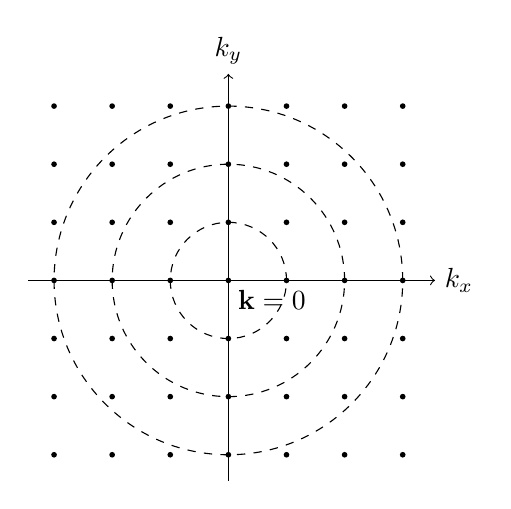
\begin{tikzpicture}[scale=0.82]
\draw[->] (-3.1,0) -- (3.2,0) node[right] {$k_x$};
\draw[->] (0,-3.1) -- (0,3.2) node[above] {$k_y$};
\draw[dashed] (0,0) circle (0.9);
\draw[dashed] (0,0) circle (1.8);
\draw[dashed] (0,0) circle (2.7);
\foreach \x in {-3,-2,-1,0,1,2,3}{
  \foreach \y in {-3,-2,-1,0,1,2,3}{
    \fill (0.9*\x,0.9*\y) circle (1.25pt);
  }
}
\node[below right] at (0,0) {$\mathbf{k}=0$};
\end{tikzpicture}
\caption{États discrets de quantité de mouvement et coquilles d’énergie constante pour des particules dans une boîte périodique finie.}
\end{figure}

Pour une particule non relativiste,
\begin{equation}
E_{\mathbf{k}}=\frac{\mathbf{k}^2}{2m},
\end{equation}
L’état d’énergie minimale est donc \(\mathbf{k}=0\). Plaçons \(N\) bosons identiques dans la boîte et cherchons leur état fondamental à plusieurs particules. Le premier boson occupe l’état d’impulsion nulle. Le deuxième peut occuper le même état, tout comme le troisième et tous les suivants. Ainsi, les \(N\) bosons occupent tous \(\mathbf{k}=0\).

Il s’agit d’un condensat de bosons : un grand nombre de particules identiques occupent le même état à une particule, ici celui d’énergie minimale. La fonction d’onde d’impulsion nulle est constante dans l’espace et s’étend à toute la boîte. Elle ne localise aucun boson en une position particulière ; la position de chacun reste donc indéterminée. Lorsque le nombre de particules dans cet état devient grand, leur fonction d’onde commune donne lieu à une amplitude de champ macroscopique, et le champ se comporte de plus en plus comme un champ classique.

L’état fondamental des fermions est tout autre. Négligeons le spin pour l’instant, de sorte que chaque point d’impulsion représente un état disponible. Le premier fermion occupe \(\mathbf{k}=0\), mais un deuxième fermion identique ne peut pas le rejoindre. Les particules suivantes doivent occuper la couche d’énergie immédiatement supérieure. Dans un dessin à deux dimensions, quatre points du réseau non nuls les plus proches ont la même énergie ; en trois dimensions, ils sont six. Une fois ces états occupés, les particules suivantes doivent remplir les couches successives.

Comme l’énergie est proportionnelle au carré de la distance à l’origine dans l’espace des impulsions, minimiser l’énergie totale revient à remplir les points occupés aussi près que possible de \(\mathbf{k}=0\), dans la limite imposée par le principe d’exclusion. Avec un grand nombre de fermions, la région occupée prend approximativement la forme d’une sphère. Sa frontière est la surface de Fermi, son intérieur est la mer de Fermi, et l’ensemble de la région remplie constitue la sphère de Fermi. À volume fini, la frontière est légèrement irrégulière, car les points disponibles forment un réseau, mais cet effet devient négligeable dans un grand système.

\begin{figure}
\centering
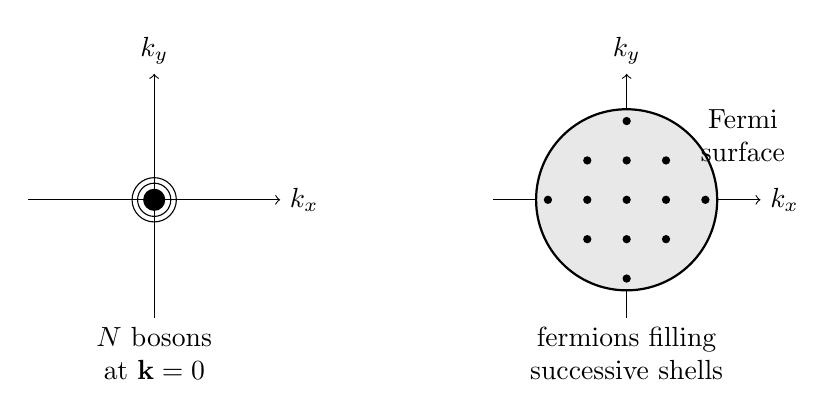
\begin{tikzpicture}[scale=1.0]
\begin{scope}[xshift=-3.0cm]
\draw[->] (-1.6,0) -- (1.6,0) node[right] {$k_x$};
\draw[->] (0,-1.5) -- (0,1.6) node[above] {$k_y$};
\fill (0,0) circle (4pt);
\draw (0,0) circle (6pt);
\draw (0,0) circle (8pt);
\node[align=center] at (0,-1.95) {$N$ bosons\\at $\mathbf{k}=0$};
\end{scope}
\begin{scope}[xshift=3.0cm]
\draw[->] (-1.7,0) -- (1.7,0) node[right] {$k_x$};
\draw[->] (0,-1.5) -- (0,1.6) node[above] {$k_y$};
\fill[gray!18] (0,0) circle (1.15);
\draw[thick] (0,0) circle (1.15);
\fill (0,0) circle (1.5pt);
\fill (0.5,0) circle (1.5pt);
\fill (-0.5,0) circle (1.5pt);
\fill (0,0.5) circle (1.5pt);
\fill (0,-0.5) circle (1.5pt);
\fill (0.5,0.5) circle (1.5pt);
\fill (0.5,-0.5) circle (1.5pt);
\fill (-0.5,0.5) circle (1.5pt);
\fill (-0.5,-0.5) circle (1.5pt);
\fill (1,0) circle (1.5pt);
\fill (-1,0) circle (1.5pt);
\fill (0,1) circle (1.5pt);
\fill (0,-1) circle (1.5pt);
\node[right,align=center] at (0.82,0.82) {Fermi\\surface};
\node[align=center] at (0,-1.95) {fermions filling\\successive shells};
\end{scope}
\end{tikzpicture}
\caption{Les bosons se condensent dans l’état de quantité de mouvement nulle, tandis que les fermions remplissent les états de quantité de mouvement de l’intérieur vers l’extérieur, jusqu’à une surface de Fermi.}
\end{figure}

L’état fondamental fermionique a une énergie bien supérieure à celle de l’état fondamental bosonique correspondant. Tous les bosons peuvent rester à impulsion nulle, mais la plupart des fermions sont contraints d’occuper des états d’impulsion non nulle. À mesure que leur nombre augmente, l’impulsion maximale occupée augmente. De plus, une couche à grande impulsion contient plus de points du réseau qu’une couche proche de l’origine. Une grande sphère de Fermi contient donc de nombreuses particules à impulsion importante et seulement quelques-unes dans les états de plus faible impulsion.

Le contraste se retrouve dans les états excités. Pour les bosons, la première excitation s’obtient en retirant un boson quelconque du condensat et en le plaçant dans un premier état excité à une particule :
\begin{equation}
(N,0,0,\ldots)\longrightarrow (N-1,1,0,\ldots).
\end{equation}
Peu importe quel boson est déplacé : les particules sont identiques. Les excitations supérieures peuvent être obtenues de plusieurs façons. Selon l’écart entre les niveaux, on peut placer un boson dans un niveau supérieur ou en placer deux dans le premier niveau excité. Exciter le système bosonique consiste à transférer des particules du condensat vers des états d’énergie supérieure.

Pour les fermions, aucune particule ne peut être déplacée vers un autre point à l’intérieur de la sphère de Fermi remplie, puisque tous ces points sont déjà occupés. Il est possible de prendre un fermion profondément enfoui dans la mer et de le placer au-dessus de la surface, mais cela coûte beaucoup d’énergie. L’excitation la moins coûteuse consiste à prendre un fermion juste à l’intérieur de la surface de Fermi et à le transférer vers un état inoccupé juste à l’extérieur. L’électron ainsi promu n’a qu’un faible excès d’énergie par rapport à la surface, et l’état vacant laissé derrière lui se trouve à peine au-dessous de celle-ci.

\begin{figure}
\centering
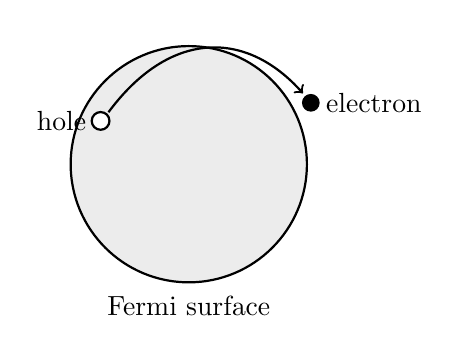
\begin{tikzpicture}[scale=1.0]
\fill[gray!15] (0,0) circle (1.5);
\draw[thick] (0,0) circle (1.5);
\draw[fill=white,thick] (-1.12,0.55) circle (3.2pt);
\fill (1.55,0.78) circle (3.2pt);
\draw[->,thick] (-1.02,0.66) .. controls (-0.25,1.7) and (0.72,1.72) .. (1.45,0.9);
\node[left] at (-1.18,0.55) {hole};
\node[right] at (1.62,0.78) {electron};
\node[below] at (0,-1.55) {Fermi surface};
\end{tikzpicture}
\caption{Une excitation fermionique de basse énergie fait passer un électron à travers la surface de Fermi et laisse un trou derrière lui.}
\end{figure}

\section{Trous et excitations de basse énergie}

Pour préciser la charge du trou, imaginons que la boîte contienne une charge positive répartie uniformément dans tout son volume. Dans la matière, cette charge positive provient en définitive des protons des noyaux, mais cette répartition uniforme simplifie le modèle. Ajoutons suffisamment d’électrons pour neutraliser ce fond. Dans l’état fondamental, ces électrons remplissent la sphère de Fermi.

Promouvoir un électron depuis un état situé au-dessous de la surface de Fermi vers un état au-dessus ne modifie pas la charge totale de la boîte. Cela crée un électron de charge négative au-dessus de la surface et laisse, au-dessous, une charge négative manquante. On peut donc traiter l’électron manquant comme une excitation de charge positive : un trou.

\begin{classroomqa}
\lecturetimestamp{01:31:38}
\audiencequestion{Un trou au-dessous de la surface de Fermi a-t-il une énergie négative ?}
\lecturerresponse{Non. Un trou est une excitation par rapport à l’état fondamental à plusieurs corps : son énergie d’excitation est donc positive. Retirer un électron occupé au-dessous de la surface de Fermi coûte une énergie positive si l’on mesure les énergies par rapport à cette surface.}
\end{classroomqa}

Soit \(\varepsilon<\varepsilon_F\) l’énergie de l’électron retiré, et \(\varepsilon'>\varepsilon_F\) celle de l’électron promu. L’énergie fournie peut se décomposer en deux écarts positifs à la surface de Fermi.\footnote{Les deux intervalles sont indiqués séparément ; l’égalité compacte présentée ici est la reformulation algébriquement équivalente.}
\begin{equation}
\Delta E
=\varepsilon'-\varepsilon
=(\varepsilon'-\varepsilon_F)+(\varepsilon_F-\varepsilon).
\end{equation}
La première contribution est naturellement attribuée à l’électron au-dessus de la surface de Fermi, et la seconde au trou au-dessous de celle-ci :
\begin{equation}
E_{\mathrm{electron}}=\varepsilon'-\varepsilon_F>0,
\qquad
E_{\mathrm{hole}}=\varepsilon_F-\varepsilon>0.
\end{equation}
L’électron porte une charge négative, et le trou une charge positive.

Un électron situé au-dessus de la surface de Fermi peut ensuite tomber dans un trou disponible. Son énergie diminue alors, et le rayonnement doit emporter l’énergie libérée. On peut décrire l’événement comme la transition d’un électron vers un état inférieur inoccupé, avec émission d’un ou de plusieurs photons. De manière équivalente, on peut dire qu’un électron et un trou s’annihilent en produisant du rayonnement. Le trou n’est pas un constituant fondamental supplémentaire de la boîte : c’est une absence dans l’état rempli de nombreux électrons. Néanmoins, son énergie et sa charge rendent utile de le traiter comme une excitation apparentée à une particule.

\begin{classroomqa}
\lecturetimestamp{01:36:52}
\audiencequestion{Promouvoir un électron signifie-t-il le déplacer d’un point du réseau à un autre dans l’espace des impulsions ?}
\lecturerresponse{Cela signifie faire passer l’électron d’un niveau d’énergie à un autre. Pour des particules libres dans la boîte, le réseau des impulsions sert à repérer ces niveaux, mais cette idée ne dépend pas d’un réseau dans l’espace des impulsions. Dans un atome, la charge positive est concentrée dans le noyau. Les électrons remplissent les niveaux atomiques disponibles les plus bas, et un photon peut faire passer un électron à un niveau excité, laissant une lacune dans le niveau qu’il occupait. Cette lacune est l’équivalent atomique d’un trou.}
\end{classroomqa}

Dans la boîte, l’absorption d’un photon convertit également son énergie en un électron au-dessus de la surface de Fermi et un trou au-dessous. Dans un atome, le même vocabulaire décrit l’électron excité et la lacune laissée parmi les niveaux inférieurs occupés.

\begin{classroomqa}
\lecturetimestamp{01:39:16}
\audiencequestion{Un photon de basse énergie peut-il être absorbé par un électron situé n’importe où dans la sphère de Fermi ?}
\lecturerresponse{Non. Si l’électron se trouve profondément dans la mer de Fermi, tous les états voisins sont déjà occupés ; un photon de basse énergie ne peut pas lui fournir assez d’énergie pour l’amener jusqu’à un état inoccupé au-dessus de la surface. Seuls les électrons suffisamment proches de la surface de Fermi ont des états vides accessibles dans la gamme d’énergie du photon. Un photon suffisamment énergétique peut exciter un électron profondément enfoui dans la mer.}
\end{classroomqa}

La section efficace d’absorption à basse énergie est donc déterminée par la surface de la mer de Fermi, et non par tout son volume. Les électrons profondément enfouis dans la mer ne peuvent pas effectuer de petites transitions ; ceux qui se trouvent juste au-dessous de la surface peuvent être transférés juste au-dessus.

\begin{classroomqa}
\lecturetimestamp{01:40:42}
\audiencequestion{Qu’est-ce qui empêche les électrons d’interagir directement entre eux, sans photon incident ?}
\lecturerresponse{Rien. Les interactions électron--électron sont négligées dans ce modèle simple, car les prendre en compte complique l’image de la mer de Fermi. Dans cette première approximation d’un métal, on considère que leur influence effective est suffisamment faible pour qu’on puisse généralement l’ignorer.}
\end{classroomqa}

\begin{classroomqa}
\lecturetimestamp{01:41:10}
\audiencequestion{Que se passe-t-il si un photon transporte assez d’énergie pour exciter plusieurs électrons ?}
\lecturerresponse{Tout processus compatible avec les lois de conservation est possible en principe. Le photon peut créer plus d’une paire électron--trou : exciter deux électrons laisse aussi deux trous. Un tel processus crée davantage d’excitations et est généralement moins probable que l’utilisation de cette énergie pour exciter beaucoup plus fortement un seul électron.}
\end{classroomqa}

\begin{classroomqa}
\lecturetimestamp{01:42:06}
\audiencequestion{Deux photons peuvent-ils être absorbés ensemble alors qu’aucun ne peut, à lui seul, produire l’excitation ?}
\lecturerresponse{Oui. L’absorption est probabiliste, et un processus à deux photons peut se produire si leur énergie combinée atteint celle d’une excitation accessible, même si l’énergie de chacun est inférieure à l’énergie requise. Si la lumière disponible ne transporte pas assez d’énergie pour atteindre une excitation autorisée, elle traverse en grande partie le système.}
\end{classroomqa}

\editorialnote{Une brève discussion à ce stade relie le rayonnement absorbé au mouvement collectif des électrons, mais ses détails de fond ne peuvent être reconstitués. Seule est établie l’affirmation selon laquelle cette réponse collective est plus complexe que le modèle à une particule--trou.}

\begin{classroomqa}
\lecturetimestamp{01:43:49}
\audiencequestion{Pourquoi les interactions électron--électron sont-elles qualifiées de faibles alors que tous les électrons portent la même charge négative ?}
\lecturerresponse{Les électrons sont plongés dans le fond positif qui compense leur charge. Ce fond écrante la charge d’un électron et réduit l’interaction effective dans ce cadre simplifié. L’interaction n’est pas absente ; pour la traiter, il faut prendre en compte la réponse d’écrantage du milieu.}
\end{classroomqa}

\begin{classroomqa}
\lecturetimestamp{01:44:41}
\audiencequestion{L’écrantage sera-t-il abordé plus loin ?}
\lecturerresponse{Oui. L’écrantage est important, mais il sera étudié lorsque le système en interaction pourra être traité plus complètement.}
\end{classroomqa}

\section{Mer fermionique à une dimension et antiparticules}

La construction du trou ouvre la voie à la notion d’antiparticule. La même structure logique peut être transposée des électrons dans la matière à un champ quantique relativiste et à son vide. La version la plus simple fait appel à un champ fermionique sans masse \(\psi(x,t)\) à une dimension spatiale. En prenant la vitesse de la lumière égale à un, les deux relations de dispersion linéaires possibles sont
\begin{equation}
\omega=k,
\qquad\text{or}\qquad
\omega=-k.
\end{equation}
Nous allons examiner explicitement la première branche.

\editorialnote{L’échange final alterne entre des identifications incompatibles des particules. Le modèle établi est un champ jouet fermionique sans masse, non spécifié, à une dimension spatiale et limité à une seule direction de propagation.}

Pour une onde plane
\begin{equation}
\psi(x,t)=e^{i(kx-\omega t)},
\end{equation}
les dérivées sont
\begin{equation}
\frac{\partial\psi}{\partial t}=-i\omega\psi,
\qquad
\frac{\partial\psi}{\partial x}=ik\psi.
\end{equation}
Ainsi, \(\omega=k\) équivaut à l’équation de champ du premier ordre
\begin{equation}
\frac{\partial\psi}{\partial t}
=-\frac{\partial\psi}{\partial x}.
\end{equation}

\begin{figure}
\centering
\includegraphics[width=0.72\textwidth]{lecture_05_figure_05.png}
\caption{On commence par établir l’équation de champ du premier ordre dont les ondes planes vérifient \(\omega=k\).}
\lectureframe{01:47:22}
\end{figure}

Tout profil de la forme \(f(x-t)\) satisfait cette équation et se propage vers la droite. En inversant le signe, on obtient
\begin{equation}
\frac{\partial\psi}{\partial t}
=+\frac{\partial\psi}{\partial x},
\end{equation}
les profils \(f(x+t)\) se propageant vers la gauche. Chacune de ces équations du premier ordre ne sélectionne qu’une seule direction de propagation. Supposons que le champ soit fermionique et, pour l’argument du trou, que ses particules portent une charge électrique.

La branche \(\omega=k\) présente une difficulté immédiate. Le nombre d’onde \(k\) peut être négatif, et \(\omega\) peut donc l’être aussi. Puisque \(\omega\) représente l’énergie dans ces unités, le spectre en droite contient des états d’énergie positive et négative :
\begin{equation}
E=\omega=k.
\end{equation}

\begin{figure}
\centering
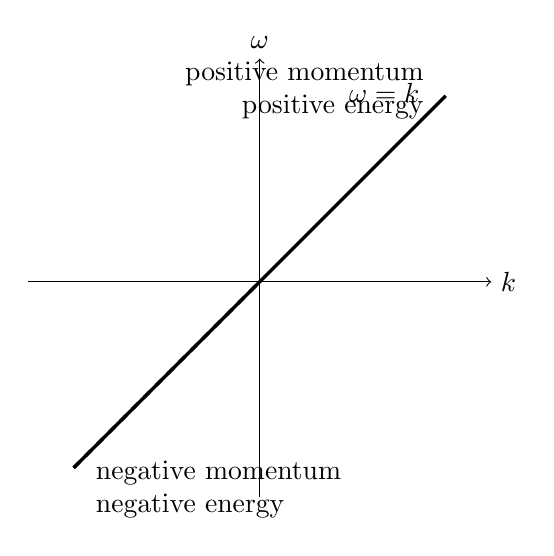
\begin{tikzpicture}[scale=1.05]
\draw[->] (-2.8,0) -- (2.8,0) node[right] {$k$};
\draw[->] (0,-2.6) -- (0,2.7) node[above] {$\omega$};
\draw[very thick] (-2.25,-2.25) -- (2.25,2.25);
\draw[very thick,dashed] (-2.25,-2.25) -- (0,0);
\node[above left] at (2.05,2.05) {$\omega=k$};
\node[below right,align=left] at (-2.1,-2.05) {negative momentum\\negative energy};
\node[above left,align=right] at (2.1,1.85) {positive momentum\\positive energy};
\end{tikzpicture}
\caption{Le spectre à une branche \(\omega=k\), dont la moitié à énergie négative se trouve pour \(k<0\).}
\end{figure}

Un vide ordinaire peut difficilement être l’état fondamental d’une telle théorie. Un fermion d’énergie positive pourrait émettre un photon et tomber vers un état inférieur. Rien ne l’obligerait à s’arrêter à zéro : il pourrait poursuivre sa descente vers des états d’énergie négative, émettre encore plus de rayonnement et tomber sans limite. L’énergie perdue par le fermion apparaîtrait dans le champ de rayonnement. Un spectre non borné inférieurement ne fournit donc pas de vide ordinaire stable.

Le principe d’exclusion des fermions offre un autre point de départ. Remplissons chaque état à une particule d’énergie négative jusqu’à l’énergie nulle, avec un fermion par état. Aucun autre fermion ne peut tomber dans ces états, puisqu’ils sont déjà occupés. Il est impossible d’ajouter un fermion d’énergie négative, tandis que l’ajout d’un fermion d’énergie positive augmente l’énergie. On peut donc prendre la mer d’énergie négative complètement remplie pour état fondamental à plusieurs corps et l’appeler le vide.

\begin{figure}
\centering
\resizebox{\linewidth}{!}{%
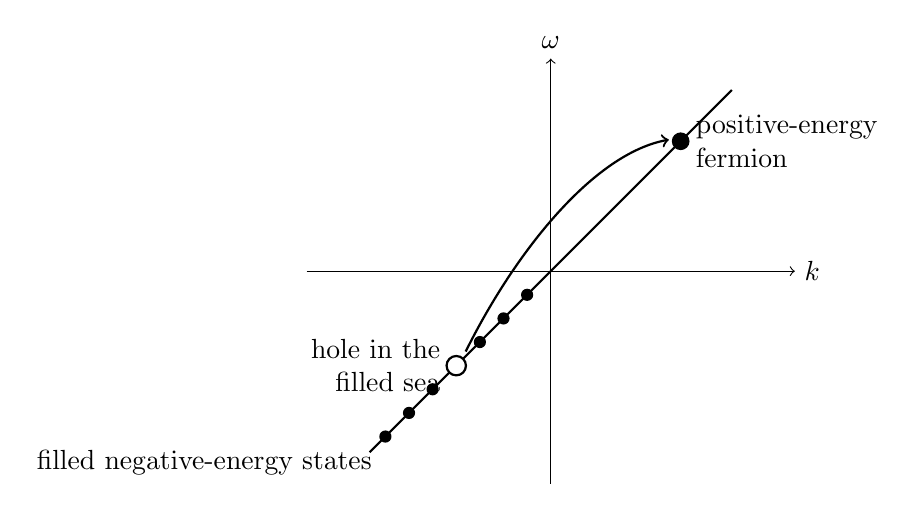
\begin{tikzpicture}[scale=1.0]
\draw[->] (-3.1,0) -- (3.1,0) node[right] {$k$};
\draw[->] (0,-2.7) -- (0,2.7) node[above] {$\omega$};
\draw[thick] (-2.3,-2.3) -- (2.3,2.3);
\foreach \p in {-2.1,-1.8,-1.5,-1.2,-0.9,-0.6,-0.3}{
  \fill (\p,\p) circle (2.2pt);
}
\draw[fill=white,thick] (-1.2,-1.2) circle (3.5pt);
\fill (1.65,1.65) circle (3.2pt);
\draw[->,thick] (-1.08,-1.02) .. controls (-0.45,0.25) and (0.55,1.5) .. (1.5,1.67);
\node[left,align=right] at (-1.28,-1.2) {hole in the\\filled sea};
\node[right,align=left] at (1.72,1.65) {positive-energy\\fermion};
\node[below left] at (-2.15,-2.15) {filled negative-energy states};
\end{tikzpicture}%
}
\caption{La mer d’énergie négative remplie et une excitation créée en faisant passer un fermion à énergie positive.}
\end{figure}

L’excitation la plus simple consiste à retirer un fermion de la mer d’énergie négative et à le placer dans un état d’énergie positive. Le fermion promu est une particule ordinaire d’énergie positive. La lacune laissée dans la mer constitue une deuxième excitation : un trou. Si le fermion retiré porte une charge négative, le trou porte une charge positive.

Dans cet exemple à une seule branche, le trou a également une impulsion positive. Si le fermion manquant occupait un état d’impulsion \(k_-<0\), son retrait modifie l’impulsion totale de
\begin{equation}
p_{\mathrm{hole}}=-k_->0.
\end{equation}
Il s’agit d’un déficit d’impulsion négative. L’excitation est donc constituée d’un fermion de charge négative et d’énergie positive, ainsi que d’un trou de charge positive et d’énergie positive. Tous deux portent une impulsion positive et, sur la branche \(\omega=k\), se propagent vers la droite.

Dans la théorie complète de l’électron, le trou de charge positive est le positon. Dirac a d’abord envisagé d’identifier le trou au proton. Cette construction exige que la particule et son antiparticule aient la même masse. Le trou est une particule distincte, de même masse que l’électron et de charge électrique opposée. C’est l’interprétation élémentaire en termes de particule--antiparticule à laquelle a conduit le spectre d’énergie négative.

On ne peut pas appliquer la même solution aux bosons. Un état bosonique peut contenir un nombre arbitraire de particules : il est donc impossible de remplir un niveau d’énergie négative une fois pour toutes et d’empêcher toute occupation supplémentaire. On peut toujours ajouter d’autres bosons à ce niveau, ce qui abaisse encore l’énergie :
\begin{equation}
\begin{aligned}
\text{fermionic mode: }&n=0\ \text{or}\ 1,\\
\text{bosonic mode: }&n=0,1,2,\ldots .
\end{aligned}
\end{equation}
Le système bosonique proposé n’aurait toujours pas d’état fondamental. Dans cette construction élémentaire, la stabilité de la mer remplie repose précisément sur le principe d’exclusion des fermions.

Cette équation à une dimension n’est qu’une version jouet de l’équation de Dirac. Son champ est sans masse, se déplace à la vitesse de la lumière et ne se propage que dans une seule direction. Une équation de Dirac plus complète doit prendre en compte les directions de mouvement manquantes ainsi que le reste de la structure relativiste de la particule. Cette équation plus complète, ainsi que le traitement des antiparticules pour les champs bosoniques, seront abordés ultérieurement.
